
\chapter{System architecture and specifications}

% În acest capitol vom începe prin a descrie care sunt obiectivele sistemului prezentat în această lucrare. 
% Continuand cu o comparatie a celor doua tipuri de arhitecturi folosite in sistemului de urmărire partilor corpului, 
% precum și detalile 
% de implementare a celor doua aplicati dezvoltate. Totodată vom pune în evidența care sunt capabilitățile aplicației.
In this chapter we will begin by describing the objectives 
of the system presented in this paper. Continuing with a comparison of the two types of architectures used 
in the body tracking system, as well as the implementation details of the two developed applications.
 At the same time, we will highlight the capabilities of the application.

\section{Goals}

\par Our motivation is to help patients who need physiotherapy to see a progress and to encourage them to be 
constant during their treatment. We want to support patients motivation in continuing to build new and 
 healthy behaviours. But also helping Physiotherapist in evaluation of patient.

% Obiectivul principal este cel de a urmari pacientul in timp ce isi face exerciti 
% ca sa ajutam kinetoterapeutul in evaluare pacientului si sa motivam pacientul prin raportarea progresului. 
The primary objective is to track the patient while he doing exercise to help 
the physical therapist in evaluation of patient and to motivate the patient by reporting progress.

% In acest sens am implementat peste algoritmul de estimare a posturi cele doua abordari detaliate in introducerea lucrari,cel care caulculeaza rang of motion si calcularea distantelor pentru afisarea progresului pacientului.

In this case, we implemented the pose estimation algorithm, 
the two approaches detailed in the introduction of the papers, 
the one that calculate Range of Motion  and the calculation of the distances for display the progress of the patient

% Dar pentru realizarea acestui obiectiv avem nevoie ca algoritmul de estimare a posturi sa aiba o performanta de minim 30 fps
% care sa poata rula atata in browser cat si pe dispozitive mobile.
But to achieve this goal, 
we need the pose estimation algorithm to have a minimum of 30 fps that can run both in the browser and on mobile devices.

% In continuare ne vom exact pe rularea algoritmilor de detectare a posturi
%  in timp real pe imagini de la camera video la o performanta de minim 30 de framuri pe secunde.
%  Dar si pe gasirea arhitecturile de retele neuronale de convolutie care sa permita acest lucru.
Next we will accurately run real-time pose estimation algorithms on the video camera at a performance of at least 30 frames per second.
  But also finding convolution neural network architectures to allow this.

%  Nu dorim folosirea unui server care sa primesca acest stream-urilor de imagini si sa aplice algoritmi de detectie
%   datorita calculelor foarte costisitoare ca timp si volumului mare de date care trebuie procesate.
We do not want to use a server that are to receive the streams of images 
and apply detection algorithms due to calculations costly in time and volume of data to be processed.

% Varianta cu servar a fost implementat dar mare problema a fost delay de 3-4 sec 
%   astfel obiectivul nostrul minim 30 de framuri pe secunda nu putea fi realizabil.
The server variant was implemented but the big problem 
was a delay of 3-4 sec so our goal of at least 30 frames per second could not be achieved.


% Pentru a obtine performance maxime a algoritmilor este necesara rularea lor pe placa grafica a aplicatie client.
To achieve maximum performance of the algorithms, 
it is necessary to run them on the GPU of the client application. 

%  Noi am propus implementare a doua prototipuri , o aplicatie web si una mobile. 
 We proposed the implementation of two prototypes, a web application and a mobile application.
%  Fiecare aplicatie implementeaza o abordarea diferite care foloseste o arhitectura defirita de retea neuronala de convolutie
Each application implements a different approach that uses a different type of architecture from convolution neural network.

%  Aplicatie web calculeaza Range of Motion pentru a ajuta pacientul sa faca corect exercitile, astfel vom numara numarul de repatari corecte pe baza unghiurilor care le optine pacientul in timpul exercitiului
The web application will calculate a range of motion to help the patient perform the correct exercises, so we will count the correct number of repetitions of an exercise based on the angles that help the patient during the exercise.


%  Aplicatia mobile va calcula distantele facute de mainile si picioarele pacientului in timpul unui exercitiu 
%  astfel generand raporte cu performanta de la o zi la alta pentru a imbunatati motivarea pacientului.

The mobile app will calculate the distance traveled by the hands and legs during an exercise that the 
patient will perform, generating reports with day-to-day performance to improve motivation of the patient.

\section{Web - Application development}


Application is an interactive software destined for patients who need physiotherapy
treatments. Our application guide patient to see how they need to make their exercises in 
a correct manner by showing Range of Motion (ROM) in real time and after allowing us to 
 count the number of movements. 
It is based on exercices, because we think that a constant and correct number of movements could be more efficient for patients then just to present them what exercices they need to do. In this manner the application guides each patient during the all period they need to follow their treatment. 


\subsection{Analysis and design}

\subsection{MobileNet \cite{DBLP:journals/corr/HowardZCKWWAA17}}
 In urma cautarilor am dat prima data peste PoseNET care promite rularea in browser folosind tensorflow js si folosind placa grafica, bazat pe relete neuronale de convolutie cu o arhitectura de tipul MobileNetv1
 
 Algoritmul posenet facut gandit de cei de la google foloseste o arhitectura de tip mobilenet, 
 deci se foloseste un arhitectura optimizata pentru mobile dar se implementeaza in javascript pentru a rula in browser.
 
 In articolul  \cite{DBLP:journals/corr/HowardZCKWWAA17} se descriu detalile de implementare.
 Ce este special la acesta arhitectura este layerul de Depthwise Separable Convolution, fata de convolutia standar care aplicatie filtrare si combinare in acelasi layer, Depthwise Separable Convolution se face in doi pasi separati ( mai citesc)
  
 \begin{figure}[htbp]
	\centerline{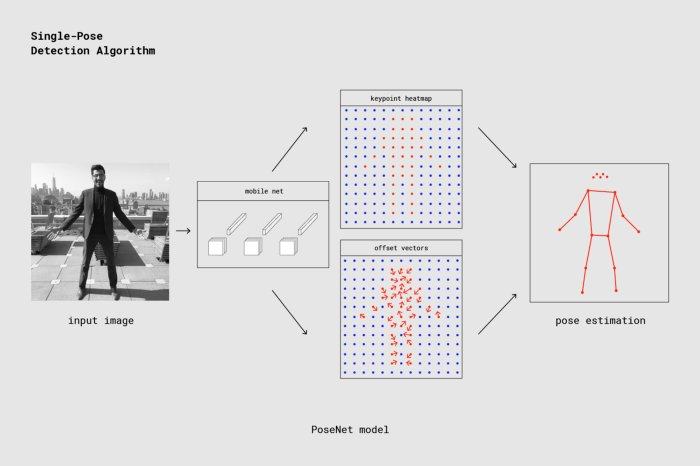
\includegraphics[scale=0.5]{fig/posenet.png}}  
	\caption{Single person pose detector pipeline using PoseNet}
	\label{fig:posenet-work}
\end{figure}
Ideei \cite{DBLP:journals/corr/HowardZCKWWAA17}
 \begin{itemize}
     \item acest tip de arhitectura se acxeaza pe performanta retelei, astfel reducand numar de compuntati
     \item  Operația de convoluție standard are efectul de filtrare a funcțiilor bazate pe kernelurile convoluționale și    combinarea caracteristicilor pentru a produce o nouă reprezentare.
         The filtering and combination steps can be split into two
        steps via the use of factorized convolutions called depthwise separable convolutions for substantial reduction in computational cost.
         Pașii de filtrare și de combinare pot fi împărțiți în două
        trepte prin utilizarea convoluțiilor factorizate numite convoluții separabile la adâncime pentru reducerea substanțială a costurilor de calcul.
    \item MobileNet has 28 layers., All layers are followed by a batchnorm [13] and ReLU nonlinearity 
    \item MobileNet models were trained in TensorFlow [1] using RMSprop [33] with asynchronous gradient descent similar
    to Inception V3 
    \item The second hyper-parameter to reduce the computational cost of a neural network is a resolution multiplier ρ
    It is the float multiplier for the depth (number of channels) for all convolution ops. The larger the value, the larger the size of the layers, and more accurate the model at the cost of speed. Set this to a smaller value to increase speed at the cost of accuracy.
    Acesta valoare se imulteste cu fiecare layer pentru a imbunatati performanta
    \item 
 \end{itemize}

\subsection{Implementation}

% \subsection{Posture tracking algorithm}

% \subsubsection{Initialization}
% Initialization is the first part of the pose tracking algorithm, where we detect the posture with posenet and for each part of the detected skelet we calculate a bounding box and detect the initial set of keypoints that we are going to track in the next steps.
% \subsubsection{Processing}
% Processing is composed from three main parts: 
% \begin{itemize}
%     \item Tracking 
%     \item Add new points 
%     \item Respawn / Reinitialization
% \end{itemize}
% This part is used to track as much as possible points detected in the first phase.

% \subsubsection{Keypoints tracking}
% \par Points detected in the first part will be used inside tracking algorithm Lucas-Kanade \cite{Lucas:1981:IIR:1623264.1623280} (function calcOpticalFlowPyrLK() from OpenCV). This algorithm fits into the Detect Track  class (DT) and makes a local search to determine the new position of the points of interest detected in the previous frame. For this algorithm to work fine, it's important to take consecutive frames that are easily modified. If we do a sudden move, this algorithm will fail to detect to detect the new position of a part or even all the points in the previous frame. For this case, the next two steps in the algorithm will try to restore the system. 
% \par The points in the system that are tracked are detected with Shi-Tomasi "Good features to track" \cite{323798}. 
% \par After we detect new position for our keypoints we have to detect the new bounding box that correspond to their new position. For this task we choose to detect the homography matrix based on old points and new points position. Based on homography matrix we calculate the perspective transformation of previous bounding box.
% \subsubsection{Add new points}
% \par Adding new points is a step for restoring the system. As we track certain points, we may lose track of some of them. In this case, to prevent destabilization of the system, we will add new key points.
% \par The system starts with a maximum number of key points. If a percentage of N of the maximum number of points is lost, then we will try to find others to replace the missing ones. 
% \par The detection of new points will be achieved with the Shi-Tomasi algorithm "Good features to track". To narrow the search space of these algorithms, their implementations in OpenCV allow the definition of a mask. \par A mask is an image size matrix in which we want to find the key points. To mark the fact that we want to search in a certain area we will set the value of 1, the mask, in that region and 0 in the rest. Applying a mask is important not only to narrow the search space but also to don\mbox{'}t keep the points detected in an area where our posture skeleton is not found. 
% \par More specifically in our application, for each bounding box built from the skelet we will add new points inside it. The calculated bounding box is used to create a mask that we can use inside the keypoints detection algorithm.
% \subsubsection{Respawn / Reinitialization}
% \par System reinitialization consists in the identification of the fact that we lost almost all of the tracked points and we are no longer able to estimate, with the remaining number of points, the skeleton posture. The algorithms used to reinitialize the posture are the ones used in the first phase. So basically from this phase if we are no longer able to track and estimate new posture of our skeleton then we go the the first step (Initialization).

% \par System reinitialization denotes that the system has been completely destabilized. Loss of a large number of points can occur either due to a sudden movement or because the tracking posture is no longer in the frame.



% \begin{figure}
% 	\centerline{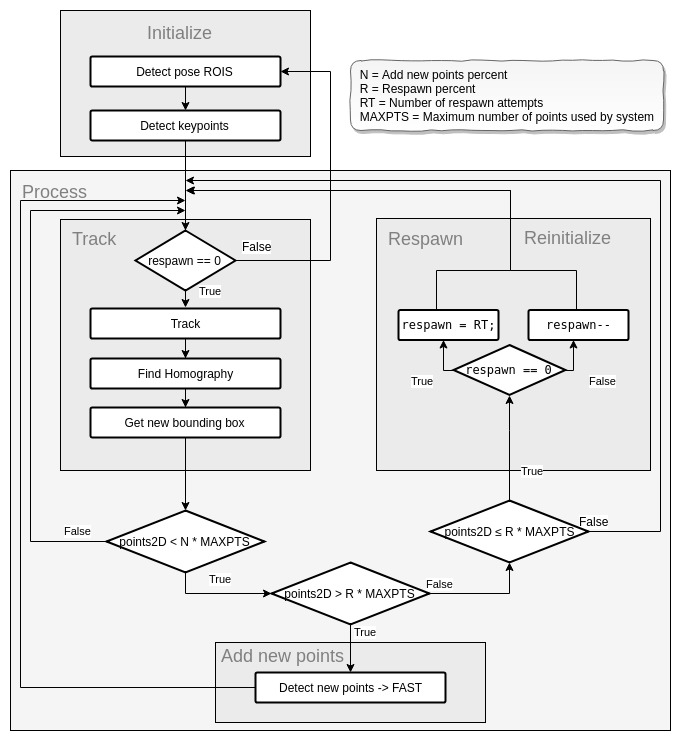
\includegraphics[scale=0.5]{fig/posture-tracking-algorithm.jpg}}  
% 	\caption{Posture tracking algorithm}
% \end{figure}


\subsection{User manual}


\section{Mobile - Application development}

\par This application is designed to help everyone who need physiotherapy treatment to stay motivated,
 reach their goals, and create habits that are healthy and helpful for a long term. 
 In this case we have a solution by creating a app which will be a useful tool for patients who needs help 
 to reach their goals by automated tracking of distances.
\subsection{Analysis and design}
\subsection{Convolutional Pose Machines \cite{DBLP:journals/corr/WeiRKS16}}
 In acest sub capitol pornim in cautarea arhitecturilor cele mai potrivite pentru pose estimation ca sa ne atinge scopul
 Deci algoritmi pe care ii gasim trebuie sa indeplinesca urmaroarele criteri
 1. Sa atinge o performanta de 30 fps pe video real time , ca acesta performanta sa fie atins trebui sa gasim o varianta de a rula pe GPU acest algoritmi
 2. Sa poata rula pe orice browser si pe orice dispozitiv mobil folosindune de camera video 
 

 
 In urma unei cautari am gasim framework tensorflow care vine cu promisiunea ca modelele lor pot 
 rula pe orice dispozitiv, astfel folosind acest framework putem rula algoritmi in browser si pe dispozitive mobile, atingandune unul dintre obiective.
 Pentru browser am gasit o implementare a frameworkului tensorflow in javascript, numit tensorflow.js.
Iar pentru mobile exista tensorflow Lite care este un model antrenat optimizat care permite rularea pe orice telefon.
 

 


Ideei \cite{DBLP:journals/corr/WeiRKS16}
\begin{itemize}
    \item Acesta arhitectura a fost special conceputea pentru pose estimation
    \item The contribution of this paper is to implicitly model long-range dependencies between variables in structured prediction tasks such as articulated pose estimation.
\end{itemize}
\subsection{Implementation}


\section{Experimental results}

\section{Possible extensions}